\chapter{Introduction}

\section{Finite state machine}
\textbf{Unified Modeling Language} is a standardized general-purpose modeling language in the field of object-oriented software engineering. The standard is managed, and was created by, the Object Management Group.\\
\url{http://www.omg.org/spec/UML}\\

\textbf{State diagram} is a type of diagram used in computer science and related fields to describe the behavior of systems. State diagrams require that the system described is composed of a finite number of states; sometimes, this is indeed the case, while at other times this is a reasonable abstraction. There are many forms of state diagrams, which differ slightly and have different semantics.\\
\url{http://en.wikipedia.org/wiki/State\_diagram}\\

\textbf{Finite state machine} is a mathematical abstraction sometimes used to design digital logic or computer programs. It is a behavior model composed of a finite number of states, transitions between those states, and actions, similar to a flow graph in which one can inspect the way logic runs when certain conditions are met. It has finite internal memory, an input feature that reads symbols in a sequence, one at a time without going backward; and an output feature, which may be in the form of a user interface, once the model is implemented. The operation of an FSM begins from one of the states (called a start state), goes through transitions depending on input to different states and can end in any of those available, however only a certain set of states mark a successful flow of operation (called accept states).\\
\url{http://en.wikipedia.org/wiki/Finite-state\_machine}\\

\begin{figure}[htbp]
    \centering
    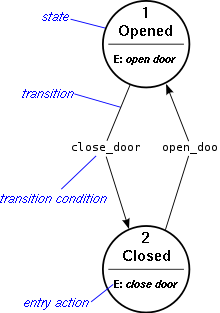
\includegraphics[scale=0.8]{images/fsm.png}
    \caption[FSM]{FSM}
\end{figure}

\textbf{The Domain Abstraction} ion of finite state machines consists of three simple elements.
\begin{itemize}
\item \textbf{States}\\
    An FSM must always be in one of several well-defined states. For example,
    the states of a simple CD player might be called Open, Empty, Stopped (with
    a CD in the drawer), Paused, and Playing. The only persistent data
    associated with a pure FSM is encoded in its state, though FSMs are seldom
    used alone in any system. For example, the parsers generated by YACC are
    built around a stack of state machines; the state of the whole system includes
    that of the stack and of each FSM in the stack.
\item \textbf{Events}\\
    State changes are triggered by events. For example in CD player example, most
    events would correspond to button presses on its front panel: play, stop,
    pause, and open/close (the button that opens and closes the drawer). Events
    aren't necessarily "pushed" into a state machine from the outside, though.
    For example, in YACC parsers, each event represents a different token, and
    is "pulled" from the input stream by the parsing process. In some systems,
    events contain associated data. For instance, an identifier token in a C++
    parser might carry the text of the identifier, while an integer-literal token
    might carry the value of the integer.
\item \textbf{Transitions}\\
    Each state can have any number of transitions to other states. Each transition
    is labeled with an event. To process an event, the FSM follows the transition
    that starts from the current state and is marked with that event. For example,
    a CD player has a transition from Playing to Stopped labeled with the stop
    event. Usually, transitions also have some associated action, such as stop
    playback in the case of our CD player. In the case of YACC, following
    transitions means manipulating the stack of FMSs and/or executing the user's
    semantic actions.
\end{itemize}

\textbf{State transition table} is a table showing what state (or states in the case of a nondeterministic finite automaton) a finite semiautomaton or finite state machine will move to, based on the current state and other inputs. A state table is essentially a truth table in which some of the inputs are the current state, and the outputs include the next state, along with other outputs.\\
\url{http://en.wikipedia.org/wiki/State\_transition\_table}\\

\begin{figure}[htbp]
    \centering
    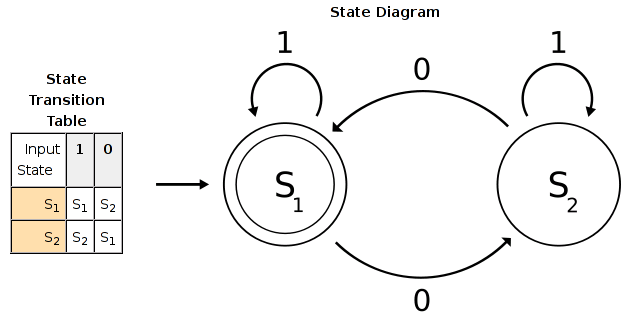
\includegraphics[scale=0.6]{images/transition_table.png}
    \caption[State transition table]{State transition table}
\end{figure}

\textbf{Virtual finite state machine} is a finite state machine (FSM) defined in a virtual environment. The VFSM concept provides a software specification method to describe the behaviour of a control system using assigned names of input control properties and of output actions. The behaviour specification is built by a state table which describes all details of a single state of the VFSM.\\
\url{http://en.wikipedia.org/wiki/VFSM}\\

\begin{figure}[htbp]
    \centering
    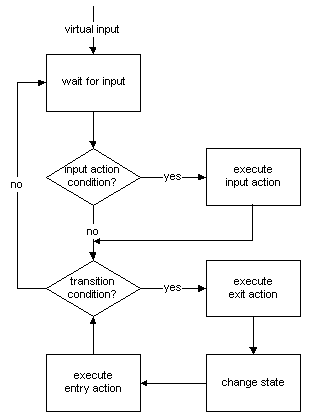
\includegraphics[scale=0.8]{images/vfsm.png}
    \caption[VFSM]{VFSM}
\end{figure}

\newpage
\textbf{State table} defines all details of the behaviour of a state of a VFSM. It consists of three columns: in the first
column state names are used, in the second the virtual conditions built out of input names using the positive logic
algebra are placed and in the third column the output names appear.\\

\begin{figure}[htbp]
    \centering
    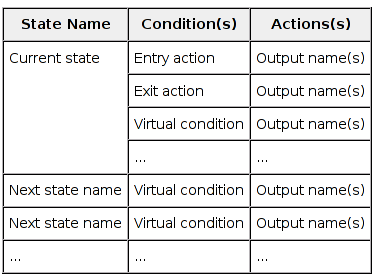
\includegraphics[scale=0.8]{images/state_table.png}
    \caption[State table]{State table}
\end{figure}

Read the table as following: the first two lines define the entry and exit actions of the current state. The following
lines which do not provide the next state represent the input actions. Finally the lines providing the next state
represent the state transition conditions and transition actions. All fields are optional. A pure combinatorial VFSM is
possible in case only where input actions are used, but no state transitions are defined. The transition action can be
replaced by the proper use of other actions.\\

